% !TEX root = main.tex

First of all, we decoded and encoded the email contents to ascii. Then we generalized the notion of word to every basic unit of characters based on whitespace and made all of characters as a list. This process is called tokenization. After creating the list of texts, we removed the stop word to reduce the noise from contents. In addition to create the list of unit characters, we also tried bag of n-grams models for uni-gram and bi-gram to count the frequency of words.\\

After having previous step, we used tf-idf to give weight of words in each email. Total number of uni-gram bag of words in training data is 1053414. We would use this tf-idf model to fit the testing data. \\\

Because the total number of email data we have is 111916. In this case, the number of features(p) is larger than the number of data set(n). Such situation will cause our features matrix becomes non-singular. Therefore, we applied the following data reduction.\\

The method we used for data reduction is called Latent Semantic Analysis (LSA) which is similar with Singular Value Decomposition (SVD). LSA can help us reduce the number of features without losing too much information. LSA also used the consine of the angle between two vectors to form the feature matrix. We reduced our features to only 100 dimensions and used reduced features matrix to fit the models.\\

In the Figure. \ref{FE}, we displayed the scatter plot of first two components. We can find out that the spam and ham email have been lightly separated.

\begin{figure}[H]
    \centering
    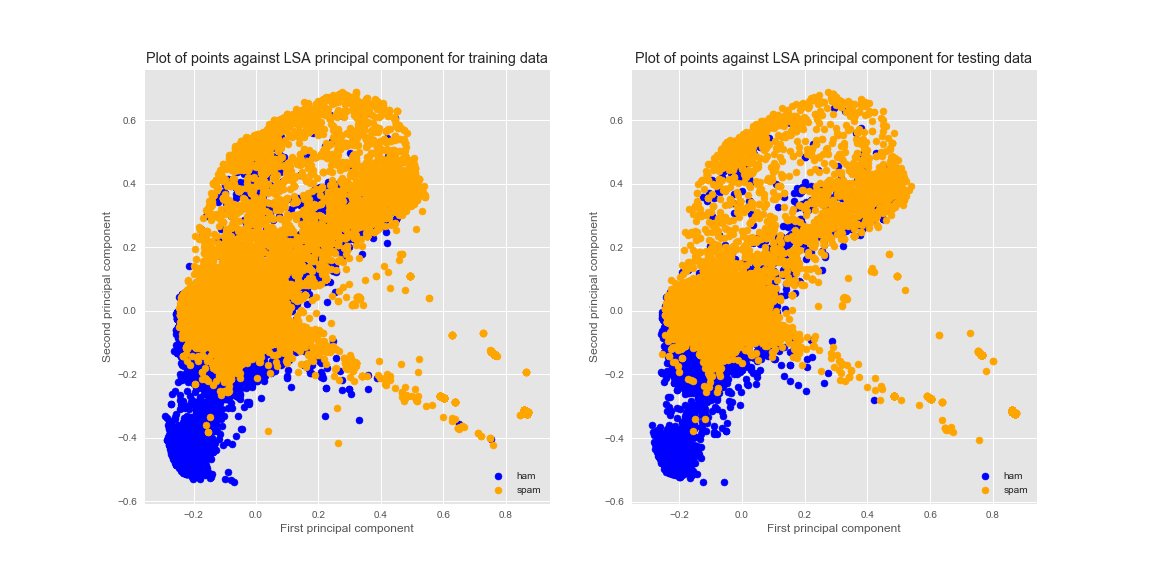
\includegraphics[scale=0.3]{./plots/data_reduction_cp12.png}
    \caption{Latent Semantic Analysis Components Plots}
    \label{FE}
\end{figure}

